
\providecommand{\sSet}{s\mathcal{S}et}%
\providecommand{\qcTwo}{\mathbf{2}}%


\section{联接与切片构造}\label{sec:the-join-and-slice-constructions}

在本节中，我们远比第 4 章中的\cref{def:join}所给出的更为详细地重访 Joyal 的%
\textbf{\trJoin}（join）与\textbf{切片}构造，并讨论它们向\trMarkedSimplicialSet{}的%
扩张。我们证明：\trMonomorphism{}以及几类\trAnodyne（anodyne）映射的 Leibniz \trJoin{}仍%
定义同种类型的\trMonomorphism。
如果我们以\emph{增广}单纯集代替通常的单纯集来工作，组合上的处理会稍微%
容易一些——这一进路沿循 Ehlers 与 Porter \cite{bib40} 对\trSimplicial\trJoin{}的原始定义。

\begin{definition}[序数和]\label{def:ordinal-sum}
代数学家的、由有限序数与保序映射构成的骨架范畴 $\Delta_{+}$——其对象为%
$[n]=\{0\le 1\le\cdots\le n\}$ 与 $[-1]=\varnothing$——承载一个严格（非对称）%
幺半结构 $(\Delta_{+},\oplus,[-1])$，其中 $\oplus$ 表示如下定义的%
\textbf{序数和}（ordinal sum）：
\begin{itemize}
\item 对对象 $[n],[m]\in\Delta_{+}$，令 $[n]\oplus[m]:=[n+1+m]$；
\item 对箭头 $\alpha\colon[n]\to[n']$、$\beta\colon[m]\to[m']$，令
$\alpha\oplus\beta\colon[n+1+m]\to[n'+1+m']$ 由
\begin{equation*}
\alpha\oplus\beta(i)=
\begin{cases}
\alpha(i) & \text{若 } i\le n,\\
\beta(i-n-1)+n'+1 & \text{否则}
\end{cases}
\end{equation*}
给出。
\end{itemize}
\end{definition}

经 Day 卷积\cite{bib33}，\trJoin\trBifunctor
$\oplus\colon\Delta_{+}\times\Delta_{+}\to\Delta_{+}$ 扩张成增广单纯集的%
\trCategory{} $\sSet_{+}:=\mathcal{S}et^{\Delta_{+}^{\mathrm{op}}}$ 上的一个%
（非对称）幺半封闭结构
\begin{equation*}
(\sSet_{+},\star,\Delta[-1],\mathrm{dec}_{l},\mathrm{dec}_{r})\mbox{.}
\end{equation*}

\begin{definition}[增广单纯集的\trJoin]\label{def:join-augmented-simplicial-sets}
增广单纯集 $X$ 与 $Y$ 的\textbf{\trJoin} $X\star Y$ 可显式描述如下：
\begin{itemize}
\item 它的诸单纯形是二元组 $(x,y)\in(X\star Y)_{r+1+s}$，其中 $x\in X_{r}$、%
$y\in Y_{s}$。
\item 设 $(x,y)$ 是 $X\star Y$ 的一个单纯形，其中 $x\in X_{r}$、$y\in Y_{s}$，%
又设 $\alpha\colon[n]\to[r+1+s]$ 是 $\Delta_{+}$ 中的一个单纯算子，则 $\alpha$%
可唯一地分解为 $\alpha=\alpha_{1}\oplus\alpha_{2}$，其中%
$\alpha_{1}\colon[n_{1}]\to[r]$、$\alpha_{2}\colon[n_{2}]\to[s]$，并且%
$(x,y)\cdot\alpha:=(x\cdot\alpha_{1},\,y\cdot\alpha_{2})$。
\end{itemize}
\end{definition}

由构造即见 $\Delta[n]\star\Delta[m]\cong\Delta[n+1+m]$，因为%
$[n]\oplus[m]=[n+1+m]$。%
\footnote{Day 卷积积的一个一般性特征是：Yoneda 嵌入%
$\mathcal{Y}\colon\Delta_{+}\hookrightarrow\mathcal{S}et^{\Delta_{+}^{\mathrm{op}}}$%
定义一个强幺半函子。}

注意 $\Delta[-1]$——即那个仅有单个 $-1$-单纯形而无其他单纯形的带标记%
\trSimplicialSet——是\trJoin\trBifunctor{}的一个双侧单位。
\footnote{译注：此处照录原书面貌。就上下文而言，$\Delta[-1]$ 作为%
$(\sSet_{+},\star)$ 的单位乃是\emph{增广}单纯集，原文作「marked simplicial
set」，疑为「augmented simplicial set」之误。}

\begin{definition}[增广单纯集的错位]\label{def:decalage}
两个闭构造 $\mathrm{dec}_{l}$ 与 $\mathrm{dec}_{r}$——分别称作\textbf{左错位%
构造}与\textbf{右错位构造}（left and right décalage constructions）——定义为%
\trJoin{}的参数化\trRightAdjoint：
\begin{center}
\begin{tikzpicture}[x=1.4em,y=1.3em]
  \node (l1) at (0,0) {$\sSet_{+}$};
  \node (r1) at (7.2,0) {$\sSet_{+}$};
  \draw[->] (1.2,0.45) to[bend left=20] node[above]{$\scriptstyle X\star-$} (6.0,0.45);
  \node at (3.6,0) {$\dashv$};
  \draw[->] (6.0,-0.45) to[bend left=20] node[below]{$\scriptstyle\mathrm{dec}_{l}(X,-)$} (1.2,-0.45);
  \node at (10.2,0) {与};
  \begin{scope}[shift={(13.2,0)}]
  \node (l2) at (0,0) {$\sSet_{+}$};
  \node (r2) at (7.2,0) {$\sSet_{+}$};
  \draw[->] (1.2,0.45) to[bend left=20] node[above]{$\scriptstyle-\star X$} (6.0,0.45);
  \node at (3.6,0) {$\dashv$};
  \draw[->] (6.0,-0.45) to[bend left=20] node[below]{$\scriptstyle\mathrm{dec}_{r}(X,-)$} (1.2,-0.45);
  \end{scope}
\end{tikzpicture}
\end{center}
从而存在由诸\trBifunctor{}构成的一个双变量伴随：
\begin{gather*}
\sSet_{+}\times\sSet_{+}
  \xrightarrow{\ -\star-\ }
\sSet_{+},\\
\sSet_{+}^{\mathrm{op}}\times\sSet_{+}
  \xrightarrow{\ \mathrm{dec}_{l}(-,-)\ }
\sSet_{+},
\qquad
\sSet_{+}^{\mathrm{op}}\times\sSet_{+}
  \xrightarrow{\ \mathrm{dec}_{r}(-,-)\ }
\sSet_{+}\mbox{.}
\end{gather*}
\end{definition}

\begin{observation}[单纯集与增广单纯集]\label{obs:ssets-vs-augmented-ssets}
遗忘增广的显然函子 $U\colon\sSet_{+}\to\sSet$ 同时容许\trLeftAdjoint{}与%
\trRightAdjoint
\begin{center}
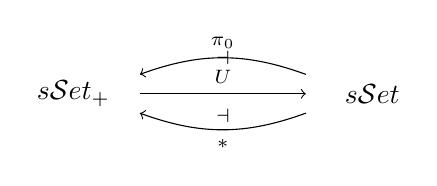
\begin{tikzpicture}[x=1.5em,y=1.4em]
  \node (l) at (0,0) {$\sSet_{+}$};
  \node (r) at (7.2,0) {$\sSet$};
  \draw[->] (5.6,0.5) to[bend right=20] node[above]{$\scriptstyle\pi_{0}$} (1.6,0.5);
  \draw[->] (1.6,0) -- node[pos=0.5,above=7pt]{$\scriptstyle\dashv$} node[above]{$\scriptstyle U$} node[pos=0.5,below=2pt]{$\scriptstyle\dashv$} (5.6,0);
  \draw[->] (5.6,-0.5) to[bend left=20] node[below]{$\scriptstyle\ast$} (1.6,-0.5);
\end{tikzpicture}
\end{center}
其中\trLeftAdjoint{}以 $\pi_{0}X$ 增广一个单纯集 $X$，这里 $\pi_{0}X$ 是由%
余等化子
\begin{equation*}
X_{1}
\;\;\mathop{\mathclap{\substack{\textstyle\delta^{1}\\\longrightarrow\\[-0.6ex]\textstyle\delta^{0}\\[-0.6ex]\longrightarrow}}}\;\;
X_{0}
\;\longrightarrow\;
\pi_{0}X
\end{equation*}
定义的路径分量集，而右伴随则通过添加单个 $-1$-单纯形来以「终」方式增广%
一个单纯集。$\pi_{0}\dashv U$ 的\trUnit{}与 $U\dashv\ast$ 的\trCounit{}都是%
\trIsomorphism；因此任一\trAdjunction{}都定义一个\trFullyFaithful{}嵌入%
$\sSet\hookrightarrow\sSet_{+}$。
\end{observation}

任何增广单纯集都典范地是其「终增广」的诸\textbf{分支}的一个\trCoproduct：
\begin{lemma}\label{lem:components-decomposition}
设 $X$ 是一个增广单纯集。
\begin{enumerate}[label=(\roman*)]
\item 对每个 $i\in X_{-1}$，由任意维数中其 $-1$-单纯形面为 $i$ 的那些单纯形%
所组成的子集 $X_{\langle i\rangle}$ 构成 $X$ 的一个终增广单纯子集。
\item 这些分支的无交并
$\coprod_{i\in X_{-1}}X_{\langle i\rangle}$ \trIsomorphism{}于 $X$。
\end{enumerate}
\end{lemma}

\begin{proof}
\cref{ex:components-decomposition-exercise}。
\end{proof}

\begin{definition}[单纯集的\trJoin]\label{def:join-simplicial-sets}
依约定，一对单纯集的\textbf{\trJoin}定义为诸平凡增广单纯集之\trJoin{}的底单纯集。
于是，\trJoin\trBifunctor{}是复合
\begin{center}
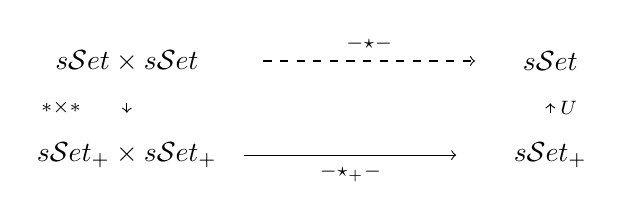
\begin{tikzpicture}[x=1.7em,y=1.7em]
  \node (tl) at (0,2) {$\sSet\times\sSet$};
  \node (tr) at (9,2) {$\sSet$};
  \node (bl) at (0,0) {$\sSet_{+}\times\sSet_{+}$};
  \node (br) at (9,0) {$\sSet_{+}$};
  \draw[->,dashed] (2.9,2) -- node[above]{$\scriptstyle-\star-$} (7.4,2);
  \draw[->] (0,1.1) -- (0,0.9);
  \node at (-1.4,1.0) {$\scriptstyle\ast\times\ast$};
  \draw[->] (9,0.9) -- node[right]{$\scriptstyle U$} (9,1.1);
  \draw[->] (2.5,0) -- node[below]{$\scriptstyle-\star_{+}-$} (7.0,0);
\end{tikzpicture}
\end{center}
显式地，$X\star Y$ 的 $n$-单纯形是由 $X$ 的一个 $j$-单纯形与 $Y$ 的一个%
$k$-单纯形组成的二元组，其中 $j+k=n-1$；当 $j=-1$ 时，这样的「二元组」
恰由 $Y$ 的单个 $n$-单纯形构成，而当 $k=-1$ 时，则恰由 $X$ 的单个%
$n$-单纯形构成。这便恢复了第 4 章中的\cref{def:join}。
\end{definition}

正如第 4 章中的\cref{def:join}所观察到的，单纯集 $X$ 与 $Y$ 的\trJoin{}容许%
典范嵌入
\begin{equation*}
X\hookrightarrow X\star Y\hookleftarrow Y
\end{equation*}
这些嵌入可理解为：把 $X\star-$ 与 $-\star Y$ 分别作用于 $\sSet_{+}$ 中在诸%
平凡增广里挑出唯一 $-1$-单纯形的那些映射 $\Delta[-1]\to Y$ 与%
$\Delta[-1]\to X$ 所得的映射。

\begin{lemma}\label{lem:join-colimits}
\begin{enumerate}[label=(\roman*)]
\item \trJoin\trBifunctor{} $-\star-\colon\sSet\times\sSet\to\sSet$ 在每个变量%
中都保持连通余极限。
\item 对任何单纯集 $X$，诸\trJoin\trFunctor
\begin{equation*}
\sSet\xrightarrow{\ X\star-\ }X/\sSet
\qquad\text{与}\qquad
\sSet\xrightarrow{\ -\star X\ }X/\sSet
\end{equation*}
保持一切\trColimit。
\end{enumerate}
\end{lemma}

\begin{proof}
在\cref{def:join-simplicial-sets}中，单纯集的\trJoin{}被定义为三个\trFunctor{}的%
复合，其中有两个\trFunctor{}拥有\trRightAdjoint，从而保持一切\trColimit。%
第三个\trFunctor{} $\ast\colon\sSet\to\sSet_{+}$ 不拥有\trRightAdjoint，但%
从下述定义看得出它仍保持\emph{连通}余极限：一个标号 $1$-\trCategory{} $J$
是连通的，当且仅当取值于单点集的常值 $J$-标号图表的余极限是单点集。这就%
证明了 (i)。

现在，\trForgetfulFunctor{} $X/\sSet\to\sSet$ 严格地创造连通余极限%
\cite[3.3.8]{bib104}，故 (ii) 中的诸\trJoin\trFunctor{}保持连通余极限。任意%
\trColimit{}都可由连通余极限与\trCoproduct{}构造出来，因此为证 (ii)，只剩%
下论证这些\trFunctor{}保持\trCoproduct。虽然若把%
$\coprod_{i}(X\star Y_{i})$ 解释为 $\sSet$ 中的余积，则%
$X\star(\coprod_{i}Y_{i})\ncong\coprod_{i}(X\star Y_{i})$，但可以直接验证：%
$X\star(\coprod_{i}Y_{i})$ 是 $\coprod_{i}(X\star Y_{i})$ 模去把每一个包含%
$X\hookrightarrow X\star Y_{i}$ 的像等同于 $X$ 的单个副本所得的商，而这恰是%
$X/\sSet$ 中余积的构造。
\end{proof}

\begin{definition}[单纯集的切片]\label{def:slices-of-simplicial-sets}
范畴 $\sSet$ 与 $X/\sSet$ 都是局部可表现的，故\cref{lem:join-colimits}(ii)%
的诸\trCocomplete{}函子都拥有\trRightAdjoint（见\cite[1.57]{bib1}），这些右%
伴随在 $f\colon X\to A$ 处的值定义了 Joyal 的\textbf{切片单纯集}（sliced simplicial
sets）${}^{f/}\!A$ 与 $A_{/f}$，它们由第 4 章中的%
\cref{prop:join-slice-adjunction}所描述的诸\trUniversalProperty{}刻画：
\begin{gather*}
\mbox{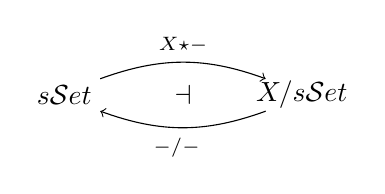
\begin{tikzpicture}[x=1.3em,y=1.3em]
  \node (l) at (0,0) {$\sSet$};
  \node (r) at (6.6,0) {$X/\sSet$};
  \draw[->] (1.0,0.45) to[bend left=20] node[above]{$\scriptstyle X\star-$} (5.6,0.45);
  \node at (3.3,0) {$\dashv$};
  \draw[->] (5.6,-0.45) to[bend left=20] node[below]{$\scriptstyle-/-\;\;{}$} (1.0,-0.45);
\end{tikzpicture}}
\qquad
\left\{\,Y\to{}^{f/}\!A\,\right\}:=
\left\{\vcenter{\hbox{\begin{tikzpicture}[x=1.2em,y=1.2em]
  \node (x) at (1.4,0.9) {$X$};
  \node (a) at (4.2,0) {$A$};
  \node (xy) at (0,-0.9) {$X\star Y$};
  \draw[->] (2.2,0.78) -- (3.8,0.25);
  \node at (3.3,0.75) {$\scriptstyle f$};
  \draw[right hook->] (1.0,0.4) -- (0.4,-0.5);
  \draw[->] (1.2,-0.9) -- (3.2,-0.35);
\end{tikzpicture}}}\right\} \\[0.8em]
\mbox{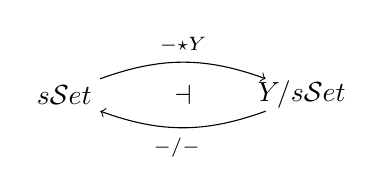
\begin{tikzpicture}[x=1.3em,y=1.3em]
  \node (l) at (0,0) {$\sSet$};
  \node (r) at (6.6,0) {$Y/\sSet$};
  \draw[->] (1.0,0.45) to[bend left=20] node[above]{$\scriptstyle-\star Y$} (5.6,0.45);
  \node at (3.3,0) {$\dashv$};
  \draw[->] (5.6,-0.45) to[bend left=20] node[below]{$\scriptstyle-/-\;\;{}$} (1.0,-0.45);
\end{tikzpicture}}
\qquad
\left\{\,X\to A_{/g}\,\right\}:=
\left\{\vcenter{\hbox{\begin{tikzpicture}[x=1.2em,y=1.2em]
  \node (y) at (1.4,0.9) {$Y$};
  \node (a) at (4.2,0) {$A$};
  \node (xy) at (0,-0.9) {$X\star Y$};
  \draw[->] (2.2,0.78) -- (3.8,0.25);
  \node at (3.3,0.75) {$\scriptstyle g$};
  \draw[right hook->] (1.0,0.4) -- (0.4,-0.5);
  \draw[->] (1.2,-0.9) -- (3.2,-0.35);
\end{tikzpicture}}}\right\}\mbox{.}
\end{gather*}
\end{definition}

我们把切片 ${}^{f/}\!A$ 想成\textbf{\trDiagram{} $f$ 之下的诸\trCone}的单纯集，
而把对偶切片 $A_{/f}$ 想成\textbf{\trDiagram{} $f$ 之上的诸\trCone}的单纯集。
这一术语与第 4 章中的\cref{def:infinity-category-of-cones}的术语之间的调和
将在\cref{prop:slices-cones-equivalence}中给出。
我们还能经由\cref{lem:components-decomposition}从\cref{def:decalage}的%
错位构造中恢复这些切片单纯集：

\begin{lemma}\label{lem:slices-as-components}
对任何单纯映射 $f\colon X\to A$，单纯集 ${}^{f/}\!A$ 与 $A_{/f}$ 分别是%
$\mathrm{dec}_{l}(X,A)$ 与 $\mathrm{dec}_{r}(X,A)$ 的、由 $-1$-单纯形%
$f\colon X\to A$ 所标引的终增广分支。
\end{lemma}

\begin{proof}
我们把单纯集 $X$ 与 $A$ 等同于它们的终增广单纯集。回顾%
$\Delta[-1]$ 是 $\sSet_{+}$ 上\trJoin\trBifunctor{}的幺半单位。于是，由%
\trAdjunction{}性，映射%
$\Delta[-1]\to\mathrm{dec}_{l}(X,A)$ 或 $\Delta[-1]\to\mathrm{dec}_{r}(X,A)$%
对应于映射 $X\to A$。对另一个终增广单纯集 $Y$，沿\cref{def:decalage}的%
\trAdjunction{}作转置便给出一个对应：
\begin{equation*}
\left\{\vcenter{\hbox{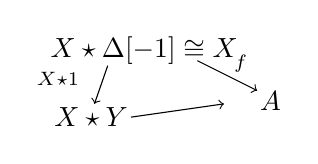
\begin{tikzpicture}[x=1.2em,y=1.2em]
  \node (t) at (1.6,1.0) {$X\star\Delta[-1]\cong X$};
  \node (a) at (5.4,-0.5) {$A$};
  \node (xy) at (0,-1.0) {$X\star Y$};
  \draw[->] (3.2,0.7) -- (5.0,-0.2);
  \node at (4.5,0.6) {$\scriptstyle f$};
  \draw[->] (0.5,0.55) -- (0.1,-0.6);
  \node at (-1.0,0.15) {$\scriptstyle X\star 1$};
  \draw[->] (1.2,-1.0) -- (4.0,-0.6);
\end{tikzpicture}}}\right\}
\cong
\left\{\vcenter{\hbox{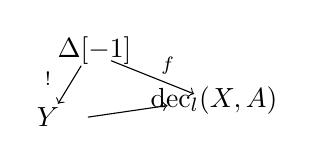
\begin{tikzpicture}[x=1.2em,y=1.2em]
  \node (t) at (1.4,1.0) {$\Delta[-1]$};
  \node (y) at (0,-1.0) {$Y$};
  \node (d) at (5.0,-0.5) {$\mathrm{dec}_{l}(X,A)$};
  \draw[->] (1.0,0.55) -- (0.3,-0.6);
  \node at (0.0,0.15) {$\scriptstyle !$};
  \draw[->] (1.9,0.7) -- (4.4,-0.3);
  \node at (3.6,0.55) {$\scriptstyle f$};
  \draw[->] (1.2,-1.0) -- (3.6,-0.65);
\end{tikzpicture}}}\right\}
\end{equation*}
这便表明 $\mathrm{dec}_{l}(X,A)$ 中由其 $-1$-单纯形面为 $f$ 的那些单纯形%
组成的单纯子集，具有定义 ${}^{f/}\!A$ 的那个\trUniversalProperty。对偶论证%
表明 $\mathrm{dec}_{r}(X,A)$ 中由其 $-1$-单纯形面为 $f$ 的那些单纯形组成的%
单纯子集，具有定义 $A_{/f}$ 的那个\trUniversalProperty。换言之，这些错位%
容许如下的、作为诸切片（终增广的）之无交并的典范分解：
\begin{equation*}
\mathrm{dec}_{r}(X,A)=\coprod_{f\colon X\to A}A_{/f}
\qquad
\mathrm{dec}_{l}(X,A)=\coprod_{f\colon X\to A}{}^{f/}\!A
\end{equation*}
\end{proof}

\begin{definition}[（左／右／内）\trAnodyneExtension]\label{def:anodyne-extensions}
\begin{itemize}
\item 对 $n\ge 1$ 与 $0\le k\le n$ 的诸\textbf{\trHorn{}包含}%
$\Lambda^{k}[n]\hookrightarrow\Delta[n]$ 之集胞腔式地生成\textbf{\trAnodyneExtension}。
\item 对 $n\ge 1$ 与 $0\le k<n$ 的诸\textbf{左\trHorn{}包含}%
$\Lambda^{k}[n]\hookrightarrow\Delta[n]$ 之集胞腔式地生成\textbf{左\trAnodyneExtension}。
\item 对 $n\ge 1$ 与 $0<k\le n$ 的诸\textbf{右\trHorn{}包含}%
$\Lambda^{k}[n]\hookrightarrow\Delta[n]$ 之集胞腔式地生成\textbf{右\trAnodyneExtension}。
\item 对 $n\ge 2$ 与 $0<k<n$ 的诸\textbf{内\trHorn{}包含}%
$\Lambda^{k}[n]\hookrightarrow\Delta[n]$ 之集胞腔式地生成\textbf{内\trAnodyneExtension}。
\end{itemize}
\end{definition}

我们把对这些映射具有右\trLifting{}性质的右类分别称为\textbf{\trKanFibration}、%
\textbf{\trLeftFibration}、\textbf{\trRightFibration}与\textbf{\trInnerFibration}。
由一个容易的直接计算：

\begin{lemma}\label{lem:leibniz-join-horn-boundary}
\emph{一个\trHorn{}包含与一个\trBoundary{}包含的 Leibniz \trJoin\trIsomorphism{}于%
单个\trHorn{}包含}：
\begin{gather*}
(\Lambda^{k}[n]\hookrightarrow\Delta[n])\mathbin{\hat{\star}}
(\partial\Delta[m]\hookrightarrow\Delta[m])
\cong
\Lambda^{k}[n+1+m]\hookrightarrow\Delta[n+1+m]\mbox{,}\\
(\partial\Delta[n]\hookrightarrow\Delta[n])\mathbin{\hat{\star}}
(\Lambda^{k}[m]\hookrightarrow\Delta[m])
\cong
\Lambda^{n+k+1}[n+1+m]\hookrightarrow\Delta[n+1+m]\mbox{.}
\end{gather*}
\end{lemma}

\begin{proof}
由于\trJoin\trBifunctor{}是序数和的 Day 卷积，且 $[n]\oplus[m]=[n+1+m]$，故%
$\Delta[n]\star\Delta[m]\cong\Delta[n+1+m]$。第一个 Leibniz 张量的定义域是%
单纯集
\begin{equation*}
\Lambda^{k}[n]\star\Delta[m]
\;\underset{\Lambda^{k}[n]\star\partial\Delta[m]}{\cup}\;
\Delta[n]\star\partial\Delta[m]\mbox{.}
\end{equation*}
我们用\cref{def:join-augmented-simplicial-sets}把它等同于%
$\Delta[n+1+m]$ 的一个单纯子集。由于 $\partial\Delta[m]$ 包含 $\Delta[m]$%
的全部余维一的面，$\Delta[n]\star\partial\Delta[m]$ 这一分支便包含%
$\Delta[n+1+m]$ 的对每个指标 $j>n$ 的第 $j$ 个面。类似地，由于%
$\Lambda^{k}[n]$ 包含 $\Delta[n]$ 的除一个之外的全部余维一面，%
$\Lambda^{k}[n]\star\Delta[m]$ 这一分支便包含 $\Delta[n+1+m]$ 的对每个指标%
$i\le n$（$i=k$ 除外）的第 $i$ 个面。于是我们看到，只缺第 $k$ 个面与那个%
$n+1+m$-单纯形，这使我们能够把这个 Leibniz \trJoin{}的定义域等同于号角%
$\Lambda^{k}[n+1+m]$。
\end{proof}

从而：

\begin{corollary}\label{cor:slices-are-quasi-categories}
\emph{若 $f\colon X\to A$ 是任一单纯映射且 $A$ 是一个\trQuasiCategory，则%
${}^{f/}\!A$ 与 $A_{/f}$ 都是\trQuasiCategory}。
\end{corollary}

\begin{proof}
由\cref{lem:slices-as-components}，为证 ${}^{f/}\!A$ 是一个%
\trQuasiCategory，只需证明增广单纯集 $\mathrm{dec}_{l}(X,A)$ 对一切内号角%
容许填充体，这里诸内号角被视为平凡增广单纯集。为此，只需解出转置后的%
\trLifting{}问题，并论证 $A$ 沿如下 Leibniz \trJoin（$n\ge 2$、$0<k<n$）%
容许扩张：
\begin{center}
\begin{tikzpicture}[x=1.6em,y=1.6em]
  \node (a) at (0,1.6) {$\Lambda^{k}[n]$};
  \node (b) at (4.8,1.6) {$\mathrm{dec}_{l}(X,A)$};
  \node (c) at (0,-1.6) {$\Delta[n]$};
  \draw[->] (1.4,1.6) -- (3.2,1.6);
  \draw[right hook->] (0,0.9) -- (0,-0.7);
  \draw[->,dashed] (0.5,-1.2) -- (3.9,1.25);
  \node at (7.4,0) {$\leftrightsquigarrow$};
  \begin{scope}[shift={(10.2,0)}]
  \node (a2) at (0,1.6) {$X\star\Lambda^{k}[n]$};
  \node (b2) at (4.8,1.6) {$A$};
  \node (c2) at (0,-1.6) {$X\star\Delta[n]$};
  \draw[->] (2.5,1.6) -- (3.7,1.6);
  \draw[right hook->] (0,0.9) -- (0,-0.7);
  \draw[->,dashed] (0.5,-1.2) -- (4.1,1.3);
  \end{scope}
\end{tikzpicture}
\end{center}
由\cref{lem:mono-epi-reedy-sset}，包含 $\varnothing\hookrightarrow X$ 由诸%
包含 $\partial\Delta[m]\hookrightarrow\Delta[m]$（$m\ge 0$）胞腔式地生成；%
而由\cref{lem:leibniz-join-horn-boundary}，这些映射与内号角包含的 Leibniz
\trJoin{}都是内\trAnodyneExtension。于是，由\cref{prop:leibniz-construction-preserves}(vii)，%
Leibniz \trJoin%
$(\varnothing\hookrightarrow X)\mathbin{\hat{\star}}(\Lambda^{k}[n]\hookrightarrow\Delta[n])$
便是\trInnerAnodyne{}的，故右上方的\trLifting{}问题容许一个解，该解经转置便定义出%
左上方\trLifting{}问题的一个解。
\end{proof}

我们的下一个目标是证明：诸切片\trQuasiCategory{}等价于 4.2 节中引入的%
诸锥\trQuasiCategory。正如该节所概述的，这一结果的关键在于\trJoin{}构造与%
第 4 章中的\cref{def:fat-join}的所谓「\trFatJoin」构造之间的一个合适的%
\trEquivalence，我们现在就把后者扩张到增广单纯集。
由\cref{lem:components-decomposition}回顾：一个增广单纯集 $X$ 典范地分解为%
诸终增广单纯集的一个余积
$X\cong\coprod_{i\in X_{-1}}X_{\langle i\rangle}$，由 $-1$-单纯形之集所标引。

\begin{definition}[增广单纯集的\trFatJoin{}与错位]\label{def:fat-join-augmented}
对增广单纯集 $X\cong\coprod_{i\in X_{-1}}X_{\langle i\rangle}$ 与%
$Y\cong\coprod_{j\in Y_{-1}}Y_{\langle j\rangle}$，它们的\textbf{\trFatJoin}由%
如下\trPushout{}构造：
\begin{center}
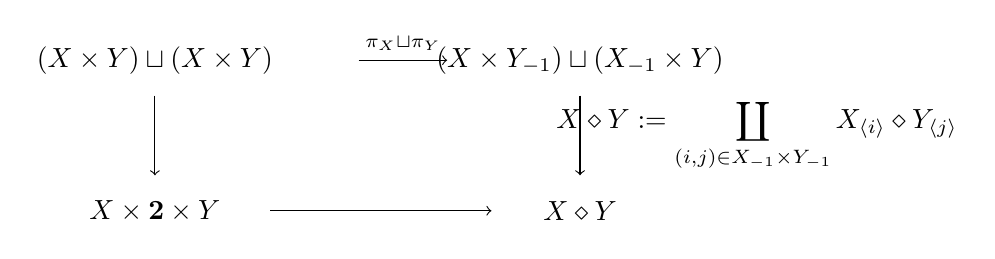
\begin{tikzpicture}[x=1.6em,y=1.6em]
  \node (tl) at (0,1.7) {$(X\times Y)\sqcup(X\times Y)$};
  \node (tr) at (9.6,1.7) {$(X\times Y_{-1})\sqcup(X_{-1}\times Y)$};
  \node (bl) at (0,-1.7) {$X\times\qcTwo\times Y$};
  \node (br) at (9.6,-1.7) {$X\diamond Y$};
  \draw[->] (4.6,1.7) -- node[above]{$\scriptstyle\pi_{X}\sqcup\pi_{Y}$} (6.6,1.7);
  \draw[->] (0,0.9) -- (0,-0.9);
  \draw[->] (9.6,0.9) -- (9.6,-0.9);
  \draw[->] (2.6,-1.7) -- (7.6,-1.7);
  \node at (3.4,0) {$\scriptstyle\ulcorner$};
  \node at (13.6,0)
    {$\displaystyle X\diamond Y:=\coprod_{(i,j)\in X_{-1}\times Y_{-1}}X_{\langle i\rangle}\diamond Y_{\langle j\rangle}$};
\end{tikzpicture}
\end{center}
其中 $X_{\langle i\rangle}\diamond Y_{\langle j\rangle}$ 是由第 4 章中的%
\cref{def:fat-join}的\trFatJoin{}所定义的终增广单纯集。这一构造的安排使得%
\trBifunctor{} $-\diamond-\colon\sSet_{+}\times\sSet_{+}\to\sSet_{+}$ 在每个
变量中都保持一切\trColimit，而不只是\trBifunctor{} $-\diamond-\colon\sSet\times\sSet\to\sSet$
所保持的那些连通余极限。
\end{definition}

显式地，$n$-单纯形之集 $(X\diamond Y)_{n}$ 是 $X\times\qcTwo\times Y$ 的%
$n$-单纯形之集 $X_{n}\times\Delta([n],[1])\times Y_{n}$ 模去如下等同三元组%
的关系所得的商：
\begin{itemize}
\item $(x,0,y)\sim(x,0,y')$，其中 $0\colon[n]\to[1]$ 是常值算子，而 $y$ 与%
$y'$ 位于 $Y\cong\coprod_{j\in Y_{-1}}Y_{\langle j\rangle}$ 的同一分支中；%
并且
\item $(x,1,y)\sim(x',1,y)$，其中 $1\colon[n]\to[1]$ 是常值算子，而 $x$ 与%
$x'$ 位于 $X\cong\coprod_{i\in X_{-1}}X_{\langle i\rangle}$ 的同一分支中。
\end{itemize}

由余连续性与伴随函子定理，$\sSet_{+}$ 上的\trFatJoin\trBifunctor{}同时拥有左闭与%
右闭 $\mathrm{fatdec}_{l}(X,A)$ 与 $\mathrm{fatdec}_{r}(X,A)$，分别称作%
\textbf{左胖错位}与\textbf{右胖错位}（left and right fat décalage）；我们%
以如下约定固定其手性：若 $X$ 是增广单纯集，则
$X\diamond-\dashv\mathrm{fatdec}_{l}(X,-)$ 且
$-\diamond X\dashv\mathrm{fatdec}_{r}(X,-)$。

从\trFatJoin{}到\trJoin{}存在一个典范的比较映射，正如围绕第 4 章中的%
\cref{prop:join-vs-fat-join}的讨论所预告的那样。

\begin{lemma}\label{lem:fat-join-comparison}
\emph{存在增广单纯集的一个典范映射
\begin{equation*}
s^{X,Y}\colon X\diamond Y\to X\star Y
\end{equation*}
它关于 $X$ 与 $Y$ 自然，特别地定义了一个\trNaturalTransformation
\begin{equation*}
s^{n,m}\colon\Delta[n]\diamond\Delta[m]\to\Delta[n]\star\Delta[m]
\qquad\in\sSet_{+}^{\Delta_{+}\times\Delta_{+}}
\end{equation*}
它在 $n$ 或 $m$ 等于 $-1$ 时是\trIsomorphism，%
\footnote{注意
$X\diamond\Delta[-1]\cong X\star\Delta[-1]\cong X\cong\Delta[-1]\diamond X\cong\Delta[-1]\star X$。}
否则则由其在顶点上的保序作用所定义的映射之商而产生：}
\begin{equation*}
\begin{aligned}
\Delta[n]\times\Delta[1]\times\Delta[m]
&\;\xrightarrow{\ \bar{s}^{n,m}\ }\;
\Delta[n+1+m]\\
(i,0,k)&\;\longmapsto\; i\\
(i,1,k)&\;\longmapsto\; k+n+1
\end{aligned}
\end{equation*}
\end{lemma}

注意 $\bar{s}^{n,m}$ 把在\cref{def:fat-join-augmented}中所描述的\trCongruence{}%
之下相关的诸单纯形送到同一个单纯形，从而在商单纯集上诱导出唯一的映射%
$s^{n,m}\colon\Delta[n]\diamond\Delta[m]\to\Delta[n]\star\Delta[m]$。在%
证明中，我们将给出映射 $s^{X,Y}$ 的一个一般构造，它可以被证明在 $X$ 与%
$Y$ 为标准单纯形的情形下与这一描述相合。

\begin{proof}
把集合 $X_{-1}$ 等同于增广单纯集
$\coprod_{X_{-1}}\Delta[-1]$，\trYonedaLemma{}提供了一个增广单纯集的典范%
映射 $X_{-1}\to X$，由此产生一个典范映射
\begin{rveq}\label{eq:fat-join-comparison-map}
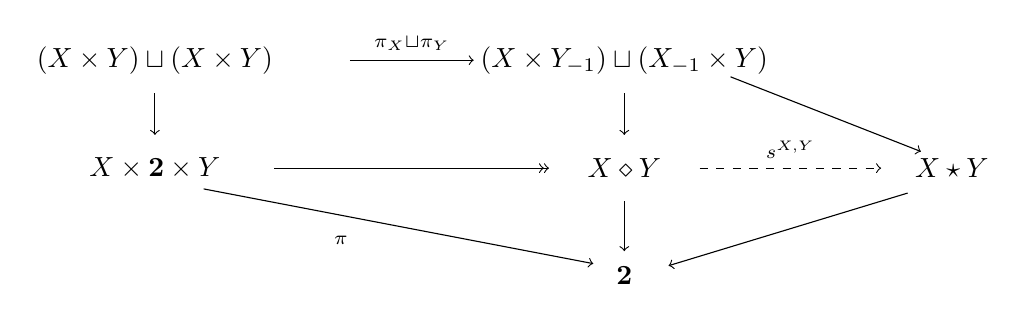
\begin{tikzpicture}[x=1.6em,y=1.5em]
  \node (tl) at (0,2.6) {$(X\times Y)\sqcup(X\times Y)$};
  \node (tr) at (10.6,2.6) {$(X\times Y_{-1})\sqcup(X_{-1}\times Y)$};
  \node (ml) at (0,0) {$X\times\qcTwo\times Y$};
  \node (mm) at (10.6,0) {$X\diamond Y$};
  \node (mr) at (18.0,0) {$X\star Y$};
  \draw[->] (4.4,2.6) -- node[above]{$\scriptstyle\pi_{X}\sqcup\pi_{Y}$} (7.2,2.6);
  \draw[->] (0,1.8) -- (0,0.8);
  \draw[->] (10.6,1.8) -- (10.6,0.8);
  \draw[->] (13.0,2.2) -- (17.3,0.4);
  \draw[->>] (2.7,0) -- (8.9,0);
  \draw[->,dashed] (12.3,0) -- node[above]{$\scriptstyle s^{X,Y}$} (16.4,0);
  \node at (9.2,0.6) {$\scriptstyle\ulcorner$};
  \node (two) at (10.6,-2.6) {$\mathbf{2}$};
  \draw[->] (1.1,-0.5) -- (9.9,-2.3);
  \node at (4.2,-1.75) {$\scriptstyle\pi$};
  \draw[->] (10.6,-0.8) -- (10.6,-2.0);
  \draw[->] (17.0,-0.6) -- (11.6,-2.35);
\end{tikzpicture}
\end{rveq}
注意 $X\diamond Y$ 与 $X\star Y$ 在 $\mathbf{2}$ 的两个端点 $0,1$ 之上的%
诸\trFiber{}分别为 $X\times Y_{-1}$ 与 $X_{-1}\times Y$，且映射 $s^{X,Y}$%
与这些\trFiber{}的包含相交换。

映射 $s^{X,Y}$ 定义在 $X\diamond Y$ 的那些映满 $\mathbf{2}$ 的 $n$-单纯形%
之上：它把代表 $X\diamond Y$ 的一个 $n$-单纯形的三元组%
$(\sigma\in X_{n},\ \alpha\colon[n]\to[1],\ \tau\in Y_{n})$ 送到代表%
$X\star Y$ 的一个 $n$-单纯形的二元组
$(\sigma|_{[0,\dots,k]}\in X_{k},\ \tau|_{[k+1,\dots,n]}\in Y_{n-k-1})$，
其中 $k\in[n]$ 是 $\alpha^{-1}(0)$ 中的最大顶点。
\end{proof}

我们现在证明：诸单纯形的\trFatJoin{}与诸单纯形的\trJoin{}之间的自然比较，定义了%
带标记\trHomotopyEquivalence{}的一个分支（见\cref{def:marked-homotopy}）。
\begin{proposition}\label{prop:comparison-marked-homotopy-retract}
\emph{对每一对 $n,m\ge-1$，增广单纯集的映射
\begin{equation*}
s^{n,m}\colon\Delta[n]\diamond\Delta[m]\longrightarrow\Delta[n]\star\Delta[m]
\qquad\in\sSet_{+}^{\Delta_{+}\times\Delta_{+}}
\end{equation*}
是一个带标记\trHomotopy{}\trRetract{}等价，并且在 $n=-1$ 或 $m=-1$ 的情形下
是一个\trIsomorphism}。
\end{proposition}

\begin{proof}
为定义 $s^{n,m}$ 的一个\trSection{}与左\trHomotopy{}逆，我们考虑一个由其在
顶点上的保序作用所确定的映射：
\begin{equation*}
\begin{aligned}
\Delta[n+1+m]\;&\xrightarrow{\ t^{n,m}\ }\;\Delta[n]\times\Delta[1]\times\Delta[m]\\
i&\;\longmapsto\;
\begin{cases}
(i,0,0) & \text{若 } i\le n,\\
(n,1,i-n-1) & \text{若 } i>n.
\end{cases}
\end{aligned}
\end{equation*}
并立即可注意到 $\bar{s}^{n,m}\bar{t}^{n,m}=\mathrm{id}$。反向的复合则由显式公式%
给出：
\begin{equation*}
\begin{aligned}
\Delta[n]\times\Delta[1]\times\Delta[m]\;&\xrightarrow{\ \bar{t}^{n,m}\bar{s}^{n,m}\ }\;\Delta[n]\times\Delta[1]\times\Delta[m]\\
(i,0,k)&\;\longmapsto\;(i,0,0)\\
(i,1,k)&\;\longmapsto\;(n,1,k)\mbox{.}
\end{aligned}
\end{equation*}
现在我们可以定义 $[n]\times[1]\times[m]$ 上的一个相关的保序自映射%
$\bar{u}^{n,m}$：
\begin{equation*}
\begin{aligned}
\Delta[n]\times\Delta[1]\times\Delta[m]\;&\xrightarrow{\ \bar{u}^{n,m}\ }\;\Delta[n]\times\Delta[1]\times\Delta[m]\\
(i,0,k)&\;\longmapsto\;(i,0,0)\\
(i,1,k)&\;\longmapsto\;(i,1,k)
\end{aligned}
\end{equation*}
这之所以引人关注，是因为在此类映射的逐点序之下我们有
$\bar{u}^{n,m}\le\bar{t}^{n,m}\circ\bar{s}^{n,m}$ 且
$\bar{u}^{n,m}\le\mathrm{id}_{[n]\times[1]\times[m]}$，它们代表诸单纯%
\trHomotopy：
\begin{center}
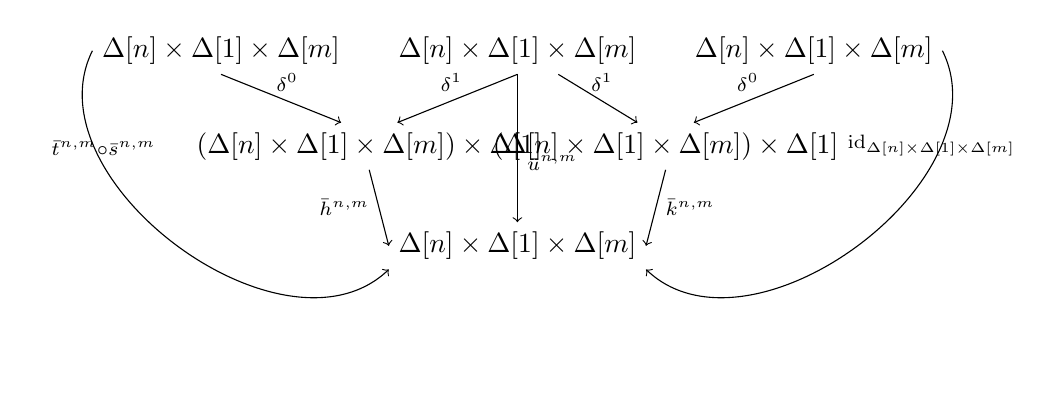
\begin{tikzpicture}[x=1.05em,y=1.5em]
  \node (A) at (0,3.4) {$\Delta[n]\times\Delta[1]\times\Delta[m]$};
  \node (B) at (10.2,3.4) {$\Delta[n]\times\Delta[1]\times\Delta[m]$};
  \node (C) at (20.4,3.4) {$\Delta[n]\times\Delta[1]\times\Delta[m]$};
  \node (L) at (5.1,1.1) {$(\Delta[n]\times\Delta[1]\times\Delta[m])\times\Delta[1]$};
  \node (R) at (15.3,1.1) {$(\Delta[n]\times\Delta[1]\times\Delta[m])\times\Delta[1]$};
  \node (D) at (10.2,-1.3) {$\Delta[n]\times\Delta[1]\times\Delta[m]$};
  \draw[->] (A.south) -- node[above,pos=0.55]{$\scriptstyle\delta^{0}$} (L.140);
  \draw[->] (B.south) -- node[above,pos=0.55]{$\scriptstyle\delta^{1}$} (L.40);
  \draw[->] (B.330) -- node[above,pos=0.55]{$\scriptstyle\delta^{1}$} (R.140);
  \draw[->] (C.south) -- node[above,pos=0.55]{$\scriptstyle\delta^{0}$} (R.40);
  \draw[->] (B.south) -- node[right,pos=0.6]{$\scriptstyle\bar{u}^{n,m}$} (D.north);
  \draw[->] (L.south) -- node[left,pos=0.5]{$\scriptstyle\bar{h}^{n,m}$} (D.west);
  \draw[->] (R.south) -- node[right,pos=0.5]{$\scriptstyle\bar{k}^{n,m}$} (D.east);
  \draw[->] (A.west) to[bend right=80] node[above,pos=0.28]{$\scriptstyle\bar{t}^{n,m}\circ\bar{s}^{n,m}$} (D.south west);
  \draw[->] (C.east) to[bend left=80] node[above,pos=0.28]{$\scriptstyle\mathrm{id}_{\Delta[n]\times\Delta[1]\times\Delta[m]}$} (D.south east);
\end{tikzpicture}
\end{center}

沿\cref{def:fat-join-augmented}所定义的同余作商，这就诱导出单纯映射%
$t^{n,m}\colon\Delta[n]\star\Delta[m]\to\Delta[n]\diamond\Delta[m]$ 与%
$u^{n,m}\colon\Delta[n]\diamond\Delta[m]\to\Delta[n]\diamond\Delta[m]$，%
使得 $s^{n,m}t^{n,m}=\mathrm{id}_{\Delta[n]\star\Delta[m]}$，以及单纯%
\trHomotopy{} $h^{n,m}$ 与 $k^{n,m}$，它们组装成如下图式：
\begin{center}
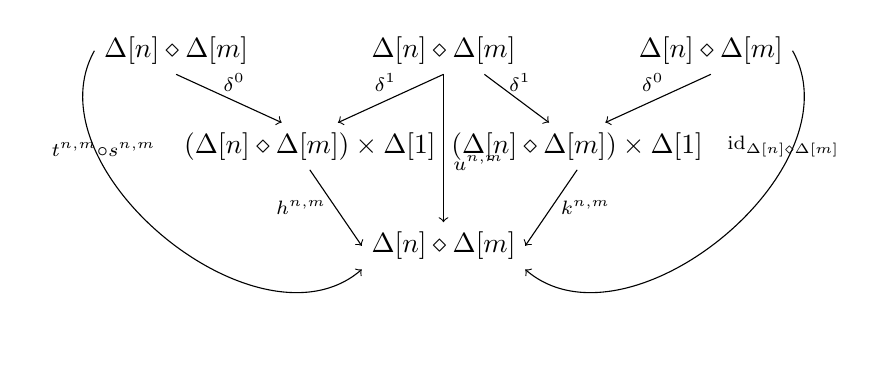
\begin{tikzpicture}[x=1.15em,y=1.5em]
  \node (A) at (0,3.4) {$\Delta[n]\diamond\Delta[m]$};
  \node (B) at (8.4,3.4) {$\Delta[n]\diamond\Delta[m]$};
  \node (C) at (16.8,3.4) {$\Delta[n]\diamond\Delta[m]$};
  \node (L) at (4.2,1.1) {$(\Delta[n]\diamond\Delta[m])\times\Delta[1]$};
  \node (R) at (12.6,1.1) {$(\Delta[n]\diamond\Delta[m])\times\Delta[1]$};
  \node (D) at (8.4,-1.3) {$\Delta[n]\diamond\Delta[m]$};
  \draw[->] (A.south) -- node[above,pos=0.55]{$\scriptstyle\delta^{0}$} (L.140);
  \draw[->] (B.south) -- node[above,pos=0.55]{$\scriptstyle\delta^{1}$} (L.40);
  \draw[->] (B.330) -- node[above,pos=0.55]{$\scriptstyle\delta^{1}$} (R.140);
  \draw[->] (C.south) -- node[above,pos=0.55]{$\scriptstyle\delta^{0}$} (R.40);
  \draw[->] (B.south) -- node[right,pos=0.6]{$\scriptstyle u^{n,m}$} (D.north);
  \draw[->] (L.south) -- node[left,pos=0.5]{$\scriptstyle h^{n,m}$} (D.west);
  \draw[->] (R.south) -- node[right,pos=0.5]{$\scriptstyle k^{n,m}$} (D.east);
  \draw[->] (A.west) to[bend right=80] node[above,pos=0.3]{$\scriptstyle t^{n,m}\circ s^{n,m}$} (D.south west);
  \draw[->] (C.east) to[bend left=80] node[above,pos=0.3]{$\scriptstyle\mathrm{id}_{\Delta[n]\diamond\Delta[m]}$} (D.south east);
\end{tikzpicture}
\end{center}

为看出映射 $h^{n,m}$ 与 $k^{n,m}$ 确实定义带标记\trHomotopy，\cref{def:marked-homotopy}
告诉我们：必须验证，对 $\Delta[n]\diamond\Delta[m]$ 的每个 $0$-单纯形%
$[i,j,k]_{\sim}$，$(\Delta[n]\diamond\Delta[m])\times\Delta[1]$ 的%
$1$-单纯形 $([i,j,k]_{\sim}\cdot\sigma^{0},\ \mathrm{id}_{[1]})$ 在%
$h^{n,m}$ 与 $k^{n,m}$ 之下被映到 $\Delta[n]\diamond\Delta[m]$ 中退化的、%
因而是带标记的单纯形。我们对指标 $j$ 分情形论证。若 $j=0$，则
$\bar{u}^{n,m}(i,0,k)=(i,0,0)=\bar{t}^{n,m}\bar{s}^{n,m}(i,0,k)$，且%
$(i,0,0)\sim(i,0,k)=\mathrm{id}(i,0,k)$，故 $h^{n,m}$ 与 $k^{n,m}$ 二者的%
分量都是退化的。
\footnote{原书印作「$(i,0,0)\sim(i,0,k)=\bar{t}^{n,m}\circ\bar{s}^{n,m}(i,0,k)$」；
按上文所列公式 $\bar{s}^{n,m}(i,0,k)=i$ 与 $\bar{t}^{n,m}(i)=(i,0,0)$，%
末端 $\bar{t}^{n,m}\bar{s}^{n,m}(i,0,k)=(i,0,0)$，疑为末端映射之名误植，%
此处径改。——译者注}
若 $j=1$，则
$\bar{u}^{n,m}(i,1,k)=(i,1,k)\sim(n,1,k)=\bar{t}^{n,m}\bar{s}^{n,m}(i,1,k)$%
\yizhu{原书此处中间项印作「$(n,i,k)$」；按上文所列公式
$\bar{t}^{n,m}\bar{s}^{n,m}(i,1,k)=(n,1,k)$，疑为中间项误植，此处径改。%
——译者注}，%
故 $h^{n,m}$ 与 $k^{n,m}$ 的分量同样都是退化的。
于是，$s^{n,m}$ 扩张成一个带标记\trHomotopy{}\trRetract{}等价，其等价逆为%
$t^{n,m}$。
\end{proof}

\cref{prop:comparison-marked-homotopy-retract}的带标记单纯%
\trHomotopyEquivalence{}见证了\cref{lem:fat-join-comparison}中所考虑的%
$\sSet_{+}^{\Delta_{+}\times\Delta_{+}}$里两个\trDiagram{}之间的、某种合适
意义下的逐点\trWeakEquivalence。这是下述证明的关键原料：增广单纯集的典范
映射 $s^{X,Y}\colon X\diamond Y\to X\star Y$ 在某种合适的意义下也是%
\trWeakEquivalence；但这一结论要求我们先探究带标记单纯集的\trHomotopy{}论
与\trQuasiCategory{}的\trHomotopy{}论之间的联系。我们将在 D.4 节中建立这一
联系，并在 D.6 节中重续这条论证线索。

我们以最后一个结果来结束本节，它是\cref{lem:leibniz-join-horn-boundary}%
的一个带标记类比。\cref{def:join-simplicial-sets}的\trJoin{}构造在\cite{bib128}
中被扩张到\trMarkedSimplicialSet。

\begin{definition}[\trMarkedSimplicialSet{}的\trJoin]\label{def:join-marked-simplicial-sets}
\trSimplicial\trJoin{}提升为一个\trJoin\trBifunctor
\begin{equation*}
\sSet^{+}\times\sSet^{+}\xrightarrow{\ \star\ }\sSet^{+}
\end{equation*}
其中，形如 $(\alpha,\beta)\colon\Delta[n]\to A\star B$ 的单纯形——其分量%
为 $\alpha\colon\Delta[k]\to A$ 与 $\beta\colon\Delta[n-k-1]\to B$——在%
$A\star B$ 中被标记，当且仅当 $\alpha$ 或 $\beta$ 至少一者在 $A$ 或 $B$ 中%
被标记。
\end{definition}

\begin{lemma}\label{lem:leibniz-join-complicial}
\begin{enumerate}[label=(\roman*)]
\item \emph{一个复状号角扩张与一个\trBoundary{}包含的 Leibniz \trJoin%
\trIsomorphism{}于单个复状号角扩张：}
\begin{equation*}
(\Lambda^{k}[n]\hookrightarrow_{r}\Delta^{k}[n])\mathbin{\hat{\star}}
(\partial\Delta[m]\hookrightarrow_{r}\Delta[m])
\cong
\Lambda^{k}[n+1+m]\hookrightarrow_{r}\Delta^{k}[n+1+m]
\end{equation*}
\emph{除非 $k=n$，此时
$(\Lambda^{n}[n]\hookrightarrow_{r}\Delta^{n}[n])\mathbin{\hat{\star}} (\partial\Delta[m]\hookrightarrow_{r}\Delta[m])$
是 $\Lambda^{n}[n+1+m]\hookrightarrow_{r}\Delta^{n}[n+1+m]$ 的一个%
\trPushout。}
\item \emph{下列诸 Leibniz \trJoin{}是复状薄性扩张}
\begin{gather*}
(\Delta^{k}[n]'\hookrightarrow_{e}\Delta^{k}[n]'')\mathbin{\hat{\star}}
(\Delta[m]\hookrightarrow_{e}\Delta[m]_{t})
\cong
\Delta^{k}[n+1+m]'\hookrightarrow_{e}\Delta^{k}[n+1+m]''\\
(\Delta^{k}[n]'\hookrightarrow_{e}\Delta^{k}[n]'')\mathbin{\hat{\star}}
(\partial\Delta[m]\hookrightarrow_{r}\Delta[m])
\cong
\Delta^{k}[n+1+m]'\hookrightarrow_{e}\Delta^{k}[n+1+m]''
\end{gather*}
\emph{除非 $k=n$，此时诸 Leibniz \trJoin{}反而是
$\Delta^{k}[n+1+m]'\hookrightarrow_{e}\Delta^{k}[n+1+m]''$ 的%
\trPushout，而
$(\Delta^{k}[n]'\hookrightarrow_{e}\Delta^{k}[n]'')\mathbin{\hat{\star}} (\Delta[m]\hookrightarrow_{e}\Delta[m]_{t})$
则是恒同映射。}
\end{enumerate}
\end{lemma}

由于\trJoin{}是反对称的——有
$(A\star B)^{\mathrm{op}}\cong B^{\mathrm{op}}\star A^{\mathrm{op}}$——
把每个 Leibniz \trJoin{}的左、右两映射相互交换而得的那些情形，都容易从这里所%
考虑的情形推得。

\begin{proof}
(i) 中作为单纯集的底映射已在\cref{lem:leibniz-join-horn-boundary}中被%
辨识，故只剩下考虑诸标记。类似地，在 (ii) 中所考虑的三个 Leibniz \trJoin{}的%
每一个里，作为单纯集的底映射都是一个\trMonomorphism{}与一个恒同的%
Leibniz \trJoin，从而是一个恒同，故只剩下考虑所得\trEntireInclusion{}中的诸标记。由于%
\trMarkedSimplicialSet{}之\trJoin{}中的一个单纯形被标记，当且仅当它的分量之一
被标记，这一描述颇便于分情形论证。我们把细节留给%
\cref{ex:finish-complicial-join-proof}或文献\cite{bib129,bib38}。
\end{proof}

\cref{def:slices-of-simplicial-sets}的切片构造也扩张到\trMarkedSimplicialSet。
我们为这一构造采用新的记号，这是因为：带标记\trJoin{}的底单纯集通常并不是底
单纯集之相应映射的切片。

\begin{lemma}\label{lem:marked-slices}
\emph{对\trMarkedSimplicialSet{}的任何映射 $f\colon X\to A$，存在由如下%
\trUniversalProperty{}刻画的\trMarkedSimplicialSet{} ${}^{f/\!/}\!A$ 与%
$A_{/\!/f}$：}
\begin{equation*}
\left\{\vcenter{\hbox{\begin{tikzpicture}[x=1.2em,y=1.2em]
  \node (x) at (1.4,0.9) {$X$};
  \node (a) at (4.2,0) {$A$};
  \node (xy) at (0,-0.9) {$X\star Y$};
  \draw[->] (2.2,0.78) -- (3.8,0.25);
  \node at (3.3,0.75) {$\scriptstyle f$};
  \draw[right hook->] (1.0,0.4) -- (0.4,-0.5);
  \draw[->] (1.2,-0.9) -- (3.2,-0.35);
\end{tikzpicture}}}\right\}
\cong
\left\{\,Y\to{}^{f/\!/}\!A\,\right\}
\qquad
\left\{\vcenter{\hbox{\begin{tikzpicture}[x=1.2em,y=1.2em]
  \node (x) at (1.4,0.9) {$X$};
  \node (a) at (4.2,0) {$A$};
  \node (xy) at (0,-0.9) {$Y\star X$};
  \draw[->] (2.2,0.78) -- (3.8,0.25);
  \node at (3.3,0.75) {$\scriptstyle f$};
  \draw[right hook->] (1.0,0.4) -- (0.4,-0.5);
  \draw[->] (1.2,-0.9) -- (3.2,-0.35);
\end{tikzpicture}}}\right\}
\cong
\left\{\,Y\to A_{/\!/f}\,\right\}\mbox{.}
\end{equation*}
\end{lemma}

\begin{proof}
\cref{ex:marked-slices-proof}。
\end{proof}

\subsection*{练习}

\begin{exercise}\label{ex:components-decomposition-exercise}
证明\cref{lem:components-decomposition}。
\end{exercise}

\begin{exercise}[{\cite{bib129,bib38}}]\label{ex:finish-complicial-join-proof}
完成\cref{lem:leibniz-join-complicial}的证明。
\end{exercise}

\begin{exercise}\label{ex:entire-inclusions-identity}
通过证明两个\trEntireInclusion{}的 Leibniz \trJoin{}是一个恒同，推广%
\cref{lem:leibniz-join-complicial}(ii)的最后一种情形。
\end{exercise}

\begin{exercise}\label{ex:marked-slices-proof}
证明\cref{lem:marked-slices}。
\end{exercise}
